\documentclass[10pt]{article}
\usepackage[a4paper,margin=2.0cm]{geometry}
\usepackage[T1]{fontenc}
\usepackage{lmodern}
\usepackage{microtype}
\usepackage{amsmath}
\usepackage{booktabs}
\usepackage{graphicx}
\usepackage{caption}
\usepackage{float}
\usepackage[hidelinks]{hyperref}
\graphicspath{{figures/}}
\setlength{\parskip}{0.45em}
\setlength{\parindent}{0pt}
\captionsetup{font=small,labelfont=bf}

\title{\vspace{-1.6em}Temporal stability: frame-to-frame flicker of LeafAlias\\ compared with the 2D CDF}
\author{}
\date{\vspace{-2.4em}}

\begin{document}
\maketitle
\vspace{-1.0em}

\textbf{Summary.} The LeafAlias partition changes from frame to frame (3--13\% of $8\times8$ cells change leaf size per frame), so we measured whether this adds flicker. It does not. Because it approximates the emitter with a few thousand leaves instead of every texel, the LeafAlias pdf changes \emph{less} between frames than the exact pdf of a 2D CDF in four of the five scenes, and equally in the fifth. In the rendered video, the low-frequency flicker (what is seen as pulsing or popping) of BudgetLeafAlias is lower than the 2D CDF's in three scenes and equal in two; relative to its per-frame error, its flicker is equal or lower in all five; after denoising it is equal or lower in all five. The coarser pdf does not cause flicker; if anything, it smooths the frame-to-frame changes of the sampling distribution.

\section*{1\quad Metrics}

On 60 consecutive frames of each of the five scenes of the paper, rendered in our GPU path tracer at equal samples, against a converged reference for every frame:
\begin{itemize}\setlength{\itemsep}{0pt}
\item \textbf{Temporal error}: $\sqrt{\langle[(I_t - I_{t-1}) - (R_t - R_{t-1})]^2\rangle}$, where $I$ is the render and $R$ the reference. Subtracting the reference's own change removes what the video itself does, so only change introduced by the renderer remains: noise and any structural flicker.
\item \textbf{Low-frequency temporal error}: the same, after a Gaussian blur with $\sigma = 8$\,px. Per-pixel noise averages out, so what remains is the kind of change seen as flicker: regions pulsing or popping between frames.
\item \textbf{Brightness pumping}: the standard deviation over frames of the mean error of the whole frame.
\item \textbf{pdf change}: the Jensen--Shannon divergence between the sampling pdfs of consecutive frames, with no rendering involved.
\end{itemize}
Rendering uses a new random seed every frame, as in normal video rendering, and we report the output both before and after the denoiser.

\section*{2\quad The coarser pdf changes less between frames}

\begin{figure}[H]
\centering
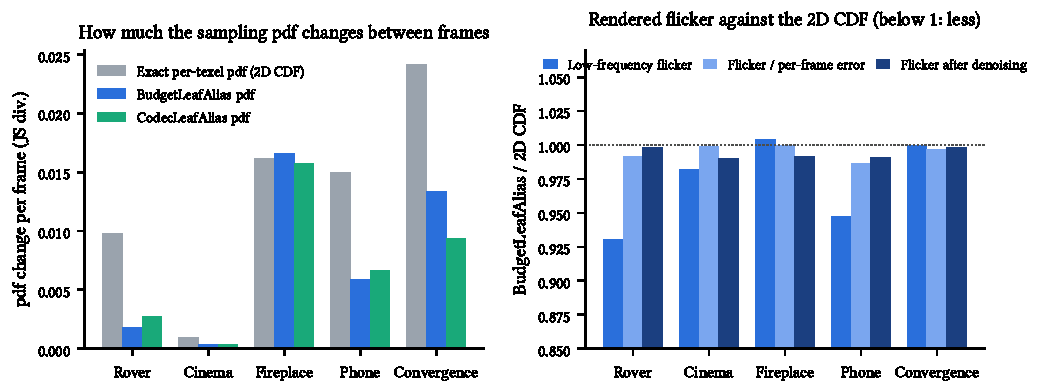
\includegraphics[width=\linewidth]{temporal_vs_cdf.pdf}
\caption{Left: how much the sampling pdf changes between consecutive frames, for the exact per-texel pdf (the 2D CDF's) and for the two LeafAlias pdfs. Right: rendered flicker of BudgetLeafAlias divided by the 2D CDF's, at equal samples; below 1 means less flicker.}
\label{fig:main}
\end{figure}

A per-texel pdf follows every change of the video, including compression noise, grain and small moving details. A leaf pdf averages each region over many texels, so these small changes largely cancel, and a leaf boundary that moves between frames only reassigns probability between neighbouring leaves of similar radiance. Figure~\ref{fig:main} (left) and Table~\ref{tab:pdf} show the result: the BudgetLeafAlias pdf changes 5.4, 2.5, 2.5 and 1.8 times less than the exact pdf in Rover, Cinema, Phone and Convergence, and about the same in Fireplace, even though 3--13\% of the cells change leaf size every frame.

\begin{table}[H]
\centering\small
\begin{tabular}{lccccc}
\toprule
& Rover & Cinema & Fireplace & Phone & Convergence \\
\midrule
pdf change per frame, exact pdf (2D CDF) & 0.0098 & 0.0010 & 0.0162 & 0.0150 & 0.0242 \\
pdf change per frame, BudgetLeafAlias & \textbf{0.0018} & \textbf{0.0004} & 0.0166 & \textbf{0.0059} & \textbf{0.0134} \\
pdf change per frame, CodecLeafAlias & \textbf{0.0027} & \textbf{0.0004} & \textbf{0.0157} & \textbf{0.0067} & \textbf{0.0093} \\
\midrule
Cells changing leaf size per frame, BudgetLeafAlias & 12.7\% & 9.9\% & 7.4\% & 13.0\% & 3.0\% \\
Cells changing leaf size per frame, CodecLeafAlias & 9.2\% & 4.4\% & 12.9\% & 9.1\% & 13.3\% \\
\bottomrule
\end{tabular}
\caption{Change of the sampling pdf between consecutive frames (Jensen--Shannon divergence, mean over 60 frames), and the share of $8\times8$ cells whose leaf size changes.}
\label{tab:pdf}
\end{table}

\section*{3\quad Rendered flicker against the 2D CDF}

\begin{table}[H]
\centering\small
\begin{tabular}{llccccc}
\toprule
& & Rover & Cinema & Fireplace & Phone & Convergence \\
\midrule
Low-frequency & 2D CDF & .0049 & .0034 & .0043 & .0027 & .0072 \\
temporal error & BudgetLeafAlias & \textbf{.0045} & \textbf{.0033} & .0043 & \textbf{.0026} & .0072 \\
& CodecLeafAlias & \textbf{.0046} & .0034 & \textbf{.0042} & .0029 & \textbf{.0071} \\
\midrule
Temporal error & 2D CDF & .0672 & .0659 & .0948 & .0377 & .1788 \\
& BudgetLeafAlias & \textbf{.0668} & .0659 & .0988 & \textbf{.0376} & .1867 \\
& CodecLeafAlias & \textbf{.0667} & .0661 & .0960 & .0382 & .1842 \\
\midrule
Temporal error / & 2D CDF & 1.315 & 1.395 & 1.331 & 1.325 & 1.326 \\
per-frame RMSE & BudgetLeafAlias & \textbf{1.303} & \textbf{1.393} & \textbf{1.330} & \textbf{1.308} & \textbf{1.322} \\
& CodecLeafAlias & \textbf{1.298} & \textbf{1.394} & 1.332 & 1.337 & \textbf{1.323} \\
\midrule
After the denoiser & 2D CDF & .0419 & .0178 & .0438 & .0230 & .0326 \\
& BudgetLeafAlias & \textbf{.0418} & \textbf{.0176} & \textbf{.0434} & \textbf{.0228} & .0326 \\
& CodecLeafAlias & .0430 & \textbf{.0177} & .0442 & .0242 & .0328 \\
\bottomrule
\end{tabular}
\caption{Flicker at equal samples, 60 consecutive frames per scene. Bold: lower than the 2D CDF.}
\label{tab:flicker}
\end{table}

\textbf{Visible flicker.} The low-frequency temporal error is the flicker a viewer sees. BudgetLeafAlias has less than the 2D CDF in Rover, Cinema and Phone (7\%, 2\% and 5\% less) and the same in Fireplace and Convergence; CodecLeafAlias is within 0.0002 of the CDF in every scene. Brightness pumping is the same for all techniques (for example 0.0027 in Cinema for all three).

\textbf{All flicker, per-pixel noise included.} The full temporal error includes the per-pixel noise of each frame, so it grows with the per-frame error. BudgetLeafAlias is equal to or below the CDF in Rover, Cinema and Phone and 4\% above in Fireplace and Convergence, the two scenes where its per-frame RMSE is also 4--5\% higher (light concentrated in small regions). Divided by the per-frame RMSE, its temporal error is lower than the CDF's in all five scenes: the partition changes add nothing measurable beyond its per-frame noise.

\textbf{After the denoiser.} The denoiser removes most per-pixel noise. What remains is equal or lower for BudgetLeafAlias in every scene.

\textbf{Structure alone.} As a diagnostic we also froze the random numbers (same seed every frame, no camera jitter), so that the image changes only through the video and the sampling structure. In that setting, where noise no longer hides it, the changing partition is visible as a fine-grained per-pixel change 1.5--3.6 times larger than the CDF's; a hierarchical warp over the same leaves brings it to 1.03--1.32 times the CDF's. This setting does not occur in normal rendering, where a new seed every frame makes this change part of the per-frame noise, as the measurements above show.

\section*{4\quad Conclusion}

The changing partition of LeafAlias does not introduce flicker. The leaf pdf changes less between frames than an exact per-texel pdf, because averaging over leaves filters out small frame-to-frame changes of the video. In the rendered output, the visible (low-frequency) flicker of BudgetLeafAlias is equal to or lower than the 2D CDF's in every scene, its flicker relative to its per-frame error is lower in every scene, and after denoising it is equal or lower in every scene. In normal rendering, using a coarser pdf approximation helps temporal stability rather than hurting it.

\end{document}
